\documentclass[12pt,twoside,a4paper]{report}
\usepackage[deti,newlogo]{uathesis}

% optional packages
\usepackage[portuguese]{babel}
\usepackage{hyperref}
\usepackage{amsmath}
\usepackage{amssymb}
\usepackage{xspace}
\usepackage{lipsum}
\usepackage{microtype}
\usepackage{multicol}
\usepackage{dirtytalk}
\usepackage{todonotes}
\usepackage[acronym,nonumberlist, nopostdot]{glossaries}
\newglossary[tlg]{nomenclature}{tld}{tdn}{Nomenclature}

\def\ThesisYear{2019}

% depth of the table of contents
\setcounter{tocdepth}{4}

% horizontal line to separate floats (figures and tables) from text
\def\topfigrule{\kern 7.8pt \hrule width\textwidth\kern -8.2pt\relax}
\def\dblfigrule{\kern 7.8pt \hrule width\textwidth\kern -8.2pt\relax}
\def\botfigrule{\kern -7.8pt \hrule width\textwidth\kern 8.2pt\relax}

\def\AddVMargin#1{\setbox0=\hbox{#1}
                  \dimen0=\ht0\advance\dimen0 by 2pt\ht0=\dimen0
                  \dimen0=\dp0\advance\dimen0 by 2pt\dp0=\dimen0
                  \box0}
\def\Header#1#2{\setbox1=\hbox{#1}\setbox2=\hbox{#2}
           \ifdim\wd1>\wd2\dimen0=\wd1\else\dimen0=\wd2\fi
           \AddVMargin{\parbox{\dimen0}{\centering #1\\#2}}}

\makenoidxglossaries
\loadglsentries{./src/glossary}

\begin{document}

% Cover pages and basic template importation requirements
%% Cover pages and basic template importation requirements
% Change with your info -------------------------------------------------

\def\theauthor{Diogo Vala \newline Correia}
\def\thesistitle{Something about Smart Shelfs, UHF RFID and Item tagging}
\def\course{Master in Electronics and Telecommunications Engineering}

\def\orientador{José Alberto Fonseca}
\def\orientadord{Associated Professor at the Departamento de Enegenharia 
Electrónica e Telecomunica\c c\~oes of the University of Aveiro}

\def\coorientador{GHI}
\def\coorientadord{Professor Catedr\'atico da Universidade de Aveiro}

\def\president{ABC}
\def\presidentd{Professor Catedr\'atico da Universidade de Aveiro}

\def\vogal{KLM}
\def\vogald{Professor Catedr\'atico da Universidade de Aveiro}

\def\frontpic{assets/frontpic.jpg}

% Abstract and acknowledgements should be edited bellow following the
% example boilerplate

% -----------------------------------------------------------------------

\def\thedeclaration{
     Dissertation submitted to the University of Aveiro in fulfillment of the thesis
     requirement for the degree of \course, under the supervision of \orientador, \orientadord 
}

\TitlePage
  \HEADER{\BAR\FIG{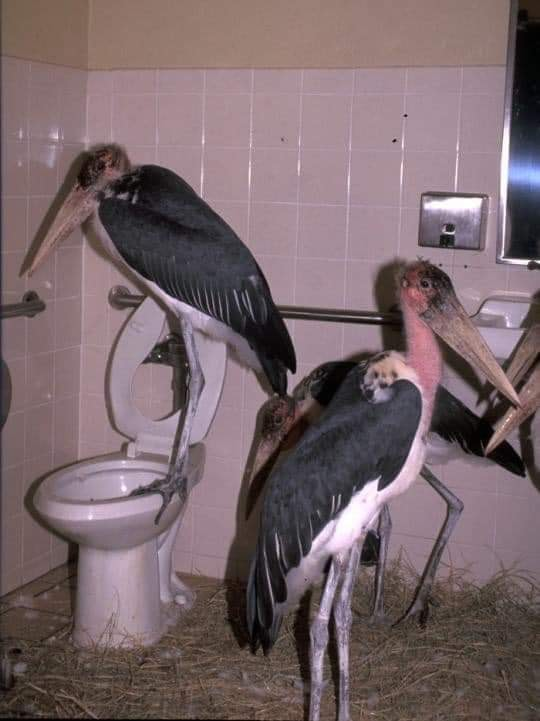
\includegraphics[height=100mm]{\frontpic}}} % the \FIG{} is optional
         {\ThesisYear}
  \TITLE{\theauthor}
        {\thesistitle}
\EndTitlePage
\titlepage\ \endtitlepage 

% Initial thesis pages
\TitlePage
  \HEADER{}{\ThesisYear}
  \TITLE{\theauthor{}}
        {\thesistitle}
  \vspace*{15mm}
  \TEXT{}
       {\thedeclaration}
\EndTitlePage
\titlepage\ \endtitlepage % empty page

\TitlePage
  \vspace*{55mm}
  \TEXT{\textbf{o j\'uri~/~the jury\newline}}
       {}
  \TEXT{presidente~/~president}
       {\textbf{\president}\newline {\small
        \presidentd \space (por delega\c c\~ao da Reitora da
        Universidade de Aveiro)}}
  \vspace*{5mm}
  \TEXT{vogais~/~examiners committee}
       {\textbf{\orientador}\newline {\small
        \orientadord \space (orientador)}}
  \vspace*{5mm}
  \TEXT{}
       {\textbf{\coorientador}\newline {\small
        \coorientadord \space (co-orientador)}}
  \vspace*{5mm}
  \TEXT{}
       {\textbf{\vogal}\newline {\small
        \vogald}}
\EndTitlePage
\titlepage\ \endtitlepage % empty page

\TitlePage
  \vspace*{55mm}
  \TEXT{\textbf{agradecimentos~/\newline acknowledgements}}
       {\'E com muito gosto que aproveito esta oportunidade para agradecer a todos os que me
        ajudaram durante este longos e penosos anos, cheios de altos e baixos (mais baixos que
        altos)\ldots}
  \TEXT{}
       {Desejo tamb\'em pedir desculpa a todos que tiveram de suportar o meu desinteresse pelas
        tarefas mundanas do dia-a-dia, \ldots}
\EndTitlePage
\titlepage\ \endtitlepage % empty page

\TitlePage
  \vspace*{55mm}
  \TEXT{\textbf{Resumo}}
       {Nos dias que correm, \'e frequente um trabalho ser avaliado pela sua apar\^encia em vez de
        o ser pelo seu conte\'udo. Sendo assim, sem descurar este \'ultimo, nesta tese descrevemos
        maneiras revolucion\'arias de transformar um documento s\'olido e austero num documento
        s\'olido e belo, capaz de fazer chorar de alegria (ou de inveja) qualquer leitor, mesmo
        quando este n\~ao percebe nada do que l\'a est\'a escrito.}
  \TEXT{}
       {A explora\c c\~ao de novas descobertas na \'area da percep\c c\~ao visual, nomeadamente
        no que se refere \`a aprecia\c c\~ao de obras de arte geniais, \ldots}
\EndTitlePage
\titlepage\ \endtitlepage % empty page

\TitlePage
  \vspace*{55mm}
  \TEXT{\textbf{Abstract}}
       {Nowadays, it is usual to evaluate a work \ldots}
\EndTitlePage
\titlepage\ \endtitlepage % empty page

% Tables of contents, of figures, ...

\pagenumbering{roman}
\tableofcontents

\cleardoublepage
\listoffigures

\cleardoublepage
\listoftables

% The chapters (usually written using the isolatin font encoding ...)

\cleardoublepage
\pagenumbering{arabic}
% Delete for release version ------------------
\pagenumbering{roman}
\tableofcontents
\printnoidxglossary[type=\acronymtype]
\addcontentsline{toc}{chapter}{\acronymname}
\printnoidxglossary
\addcontentsline{toc}{chapter}{\glossaryname}
\pagenumbering{arabic}
% ---------------------------------------------

% Import here your chapters
\chapter{Introduction}

\section{Motivation: stocks control in warehouses in mall shops and in schools (space, different operators, number of operations)}

\section{Dissertation organization (to do later)}

%\section{Context}

Nespresso is owned by Nestlé Nespresso S. A., one operational 
unit of the Nestlé Group, with headquarters in Lausanne, 
Switzerland~\cite{nespressowebsite}. (...)

The proposed solution is a system around \textbf{smart shelving}. 

The structure storing the products contains RFID antennas and 
readers that detect and read the tags attach to them. Those 
readers will let the platform know in real time the state of 
the product in stock.

This system should handle the registration and verification 
of arriving stock and manage in real time warehouse products. 

The product should integrate with the logistics management 
software used by the company, allowing the a real-time 
management off all the products, machine learning predictions 
and control of the product flow.

The solution must be reliable and cheap to maintain. The 
initial investment should also be the smallest possible. 

%\section{Motivation}

With the growing of the brand, the complexity in the logistics 
networks starts to compromise the management of the products 
down in the chain. 

The categorization and verification of new inventory, inspection 
of the arrived goods from the transportation company, returns, 
control and management of stocks, are all attended by manual 
labour. 
The manual labour is prone to errors, takes a lot of working 
time and interfacing with the management software isn't usually 
efficient.

%\section{Objectives}

\begin{itemize}
  \item \textbf{Prevent stock-outs:} get timely replenishment 
  and optimizes in-store sales and management. Logistics 
  companies deliver goods on time and according to delivery 
  requirements;
  \item \textbf{Reduce time and errors from manual labour:} 
  counts, identification, misplacement and lost or stolen items;
  \item \textbf{Help customers:} find and engage with the 
  products they want;
  \item \textbf{Control:} who removes or checks out valuable 
  items;
  \item \textbf{Automatic information and management of stock:} 
  the logistics lines automatically transmits and receives 
  stock information;
  \item \textbf{Smart physical storage:} automatic 
  identification of goods in the warehouse/shelves, 
  automatic matching of distribution requirements, improves 
  the efficiency of goods storage;
  \item \textbf{Acquisition technology:} After the goods enter 
  the collection area, the collection equipment automatically 
  identifies multiple items by collecting RFID tags, thereby 
  efficiently completing the goods in and out of the warehouse, 
  ensuring whether the physical and distribution requirements 
  are consistent, and improving the efficiency of goods 
  distribution;
  \item \textbf{Real-time:} master the distribution of all 
  goods in real time, accurately grasp the inventory situation, 
  optimize the reasonable inventory, and grasp the status and 
  changes of the warehouse environment in real time;
\end{itemize}

%\cleardoublepage
\chapter{Basic principles of RFID}

\section{History of RFID}
\section{RFID System}
\section{Tag}
\todo[inline]{Passive, Active, Semi-active; Near-field (Inductive coupling), Far-field (Backscatter coupling)}

\section{Antenna}
\todo[inline]{Overview and Information on UHF RFID Antennas and Considerations}

\section{Reader}
\section{Software and Communication Infrastructure}
\section{Technologies}
\todo[inline]{LF, HF, UHF, Microwave; Material types properties (lucent, absorbent, opaque)}

\section{Advantages and Limitations}
\chapter{EPCglobal Architecture Framework}

\section{Overview}
\todo[inline]{Activities, Standards, Goals}

\section{Global Standardization}

\subsection{Importance}

\todo[inline]{The importance of a end-to-end architecture standard (enables comunication between every member in the value chain)}

\subsection{Efforts}

Standardization of \gls{UHF RFID} for item level tagging and \gls{supply chain}, by organizations like \gls{GS1}, provided a common language to identify, capture and share supply chain data, ensuring important information is accessible, accurate and easy to understand~\cite{anonymousStandardsGS12014}.

The first prominent adoption was by the \gls{DoD} with a policy released on July 30th 2004. The policy stated that contracts issued for material delivery would require the use of RFID tags. The policy was later extended to all commodities and commodities pallets shipped to any \gls{DoD} facility~\cite{DoDSuppliersPassive, DODReleasesFinal}.

In 2014, Impinj, Intel, Google and Smartrac, joined forces to create the \gls{RAIN RFID} alliance~\cite{TechnologyCompaniesCreate} after the ratification of \gls{GS1}'s \gls{UHF RFID} Generation 2 version 2 standard in November of 2013. The alliance promotes the universal adoption of \gls{GS1}'s Gen2 \gls{UHF RFID} technologies and the connection with \gls{cloud computing}, where RFID-based data can be stored, managed and shared via the Internet~\cite{WhatRAINRFID}.
The alliance fortified the adoption of \gls{GS1}'s standards and traced a common path for the the industry to progress.

On October 11th 2018 the European Commission published their positive implementation of the upper band in Europe~\cite{302208v030101pPdf}.
It extended the power levels to $2W$ in the lower band and added the requested global band from $915$MHz to $921$MHz with power levels up to $4W$. 
This was the biggest effort by the European Commission to establish a global standardized frequency band for \gls{UHF RFID} \gls{supply chain} applications.

\subsection{Current Problems}

There are still \gls{RFID} tags that do not conform with the international standards, often presenting proprietary formats and even encoding errors.
These closed practices and struggle for market supremacy around \gls{UHF RFID} creates a problematic situation that prevent conformity through the global logistics market.

Even in global standards, the adoption depends on the company and field of business. Usually one identification standard is already being used, and the migration cost for supporting multi-code integration can be high.

The information around global standards is also limited and hard to get through. It is divided in multiple specifications, identified with number notation and codification nomenclature. 
The ISO standards, in specific, are closed and have to be payed before even see it's contents.
These specifications are extensive and don't provide newcomers a good experience. 
Companies planning to implement \gls{UHF RFID} systems following legitimate global standardization resort to consultants who have a deep knowledge on the standards complexity.

The closed mentality in the area slowed the industry progression. In comparison with the cloud and web industries, where experience and software is shared and open-sourced, \gls{UHF RFID} tends to keep everything closed. The existent freely available software is old, outdated and out of maintenance. Experience from real-world implementations is unavailable making the industry prone to committing recurrent mistakes. This results in high investments in time and money on engineering resources that could be shared among industry leaders.

The positive implementation of the upper band frequency in Europe for global \gls{UHF RFID} \gls{supply chain} applications is also dependent on the acceptance by each European members. In particular, Germany and Netherlands are not accepting it~\cite{EUUpperBand}. The conflict with existing adopted bands in the countries makes a global homogeneous system a challenge that will need time to establish.

\section{GS1 and EPCglobal}

The GS1 is a nonprofit organization dedicated to the development and implementation of standards for global \gls{supply chain} solutions. 
The institution mission is to manage the GS1 System of Standards, create open, global, multi-sector standards fostering good business practices.

GS1 established itself in 2005 from the \gls{EAN} International, \gls{UCC} and other local organizations from the United States~\cite{PublicationLEBENSMITTELZEITUNGa}.
The organization took under its umbrella the former EAN-UCC roles subsuming their technologies. From those, worth mentioning: the barcode identification system (from \gls{EAN}), \gls{XML} standards, \gls{EDI} transaction sets and \gls{supply chain} solutions~\cite[p.~212]{lahiriRFIDSourcebook2005}.

The new GS1 organization then adopted much more ambitious projects, developing global standards and services for business communication.
From those efforts resulted the network for the synchronization of master data \gls{GDSN}, the \gls{EPC} integration for \gls{RFID}, traceability and the upstream integration of the consumer goods industry suppliers and EPCglobal Network.

For RFID Technology to become viable in practice, an infrastructure must exist for processing and communicating EPC data. In meeting the goal of creating a common infrastructure, MIT announced Auto-ID Release 1.0 in October 2003. At the same time, MIT entered into an exclusive licensing agreement with GS1.
In turn, GS1 established a new division called EPCglobal to implement Release 1.0 and to conduct further development based on industry input. This put forth an initial set of standards that formed the basis of an infra- structure for EPC data. Later, Auto-ID Release 1.0 became the starting-point for the EPCglobal Network~\cite[p. 50]{GlobalRFIDValue}. 
\todo[color=red, inline]{rewrite}

\todo[inline]{EPCglobal Spec history and context}

\section{Foundations and Technical Principles}

\todo[inline]{EPC Uniqueness, Identifiers, Decentralized Implementation, Issuing Organization, \dots}
\todo[inline]{Review text - it is from and ex subsection prior to the revision of the new index}

EPCglobal Architecture Framework is a collection of interrelated hardware, software, and data standards (\emph{EPCglobal Standards}) that interoperate with shared network services (\emph{EPC Network Services}) operated by GS1, its delegates, and others~\cite{Architecture6framework20140414Pdf}.

The existence of this standards promotes not only the global adoption of \gls{EPC}, but also the exchange of information between business partners. 

The fact that the \emph{EPCglobal Framework} only defines standards for interfaces and data, frees the market of \emph{information systems} to create custom business solutions. Manufacturing can have their custom business logic closed and expose production state information to the clients through the \emph{EPCglobal} standards.

The architecture establishes three core requirements and activities, all of which have a group of standards within the \emph{EPCglobal Architecture Framework}.

\paragraph{Physical Object Exchange} 

\emph{Identify} individual products, cases, loads, assets, return items, among others, so they can be tracked individually.
The \emph{End Users} parties in a supply chain that exchange physical objects that are identified with \gls{EPC}.
Physical object exchange consists in operations such as shipping, receiving goods, and so on.
For many End Users, the physical objects are trade goods, but this could not be the case.
There are many other uses, like library or asset management applications~\cite{dong-yingliDesignInternetThings2016} that differ from the \gls{supply chain} trade goods model, but still involve the requirement for unique identification and tagging of objects. 
The architecture must be designed to ensure that when one end user delivers a physical object to another end user, the latter will be able to determine the \gls{EPC} of the physical object and interpret it properly~\cite{Architecture6framework20140414Pdf}.
The \emph{EPCglobal Architecture Framework} defines \gls{EPC} physical object exchange standards.

\paragraph{Infrastructure for Data Capture} 

\emph{Capture data} about the movement of physical assets and creating visibility.
In order to have gather \gls{EPC} data, each \emph{End User} carries out operations within its environment. That can be the creation of \gls{EPC}s for new objects, follow the movements of objects by sensing their \gls{EPC}s, and gather that information into systems of record within the organization~\cite{Architecture6framework20140414Pdf}. The \emph{EPCglobal Architecture Framework} defines interface standards for the major infrastructure components required to gather and record \gls{EPC} data. This allows \emph{End Users} to develop their internal systems using interoperable components.

\paragraph{Data Sharing} 

\emph{Exchange data} with \gls{IT} applications and trading partners, to turn visibility into information and action.
\emph{End Users} benefit from the \emph{EPCglobal Architecture Framework} by sharing data with each other, increasing the visibility they have with respect to the movement of physical objects through the \gls{supply chain}. 
The \emph{EPCglobal Architecture Framework} defines \gls{EPC} data sharing standards, which provide a means for end users to share data about \gls{EPC}s within defined user groups or with the general public, and which also provide access to \emph{EPC Network Services} and other shared services that facilitate this sharing. \todo{change phrasing a bit}

\begin{figure}[!ht]
    \centering
    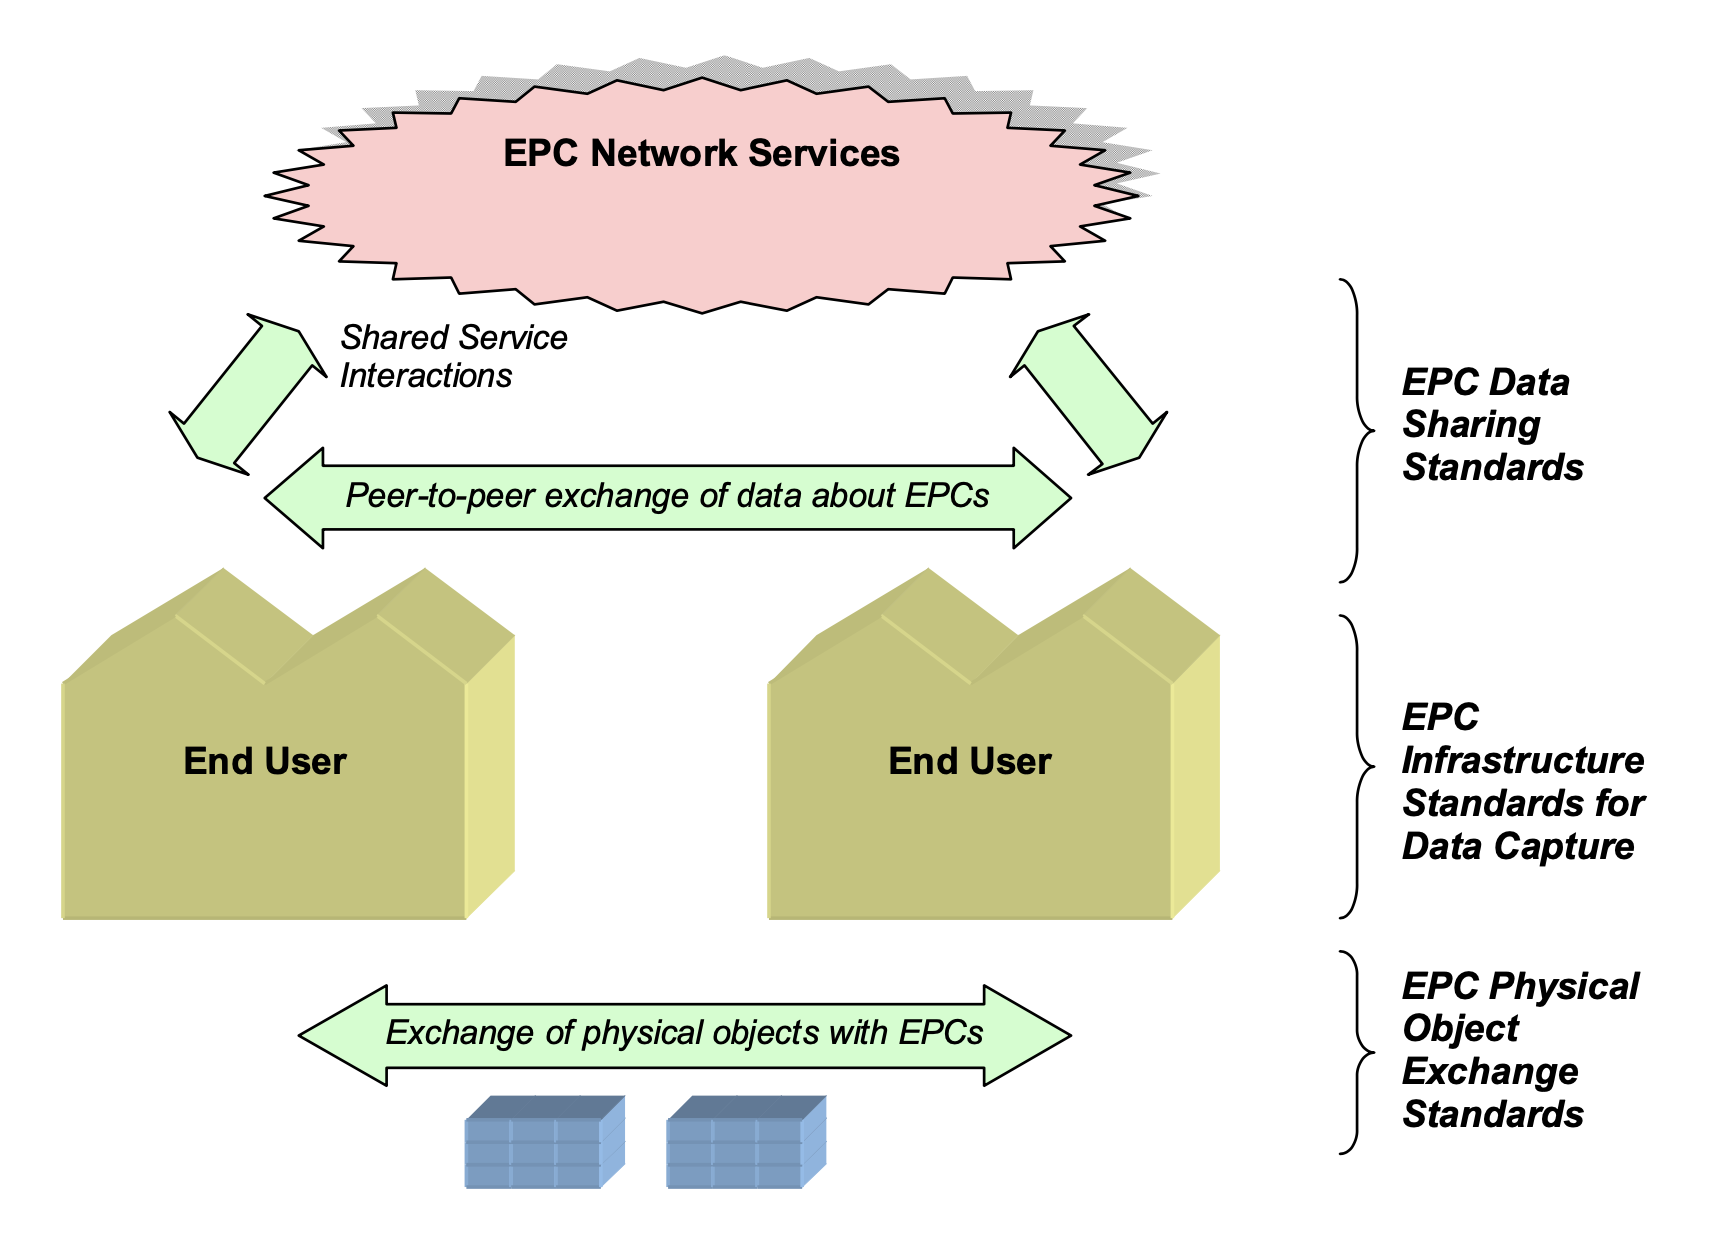
\includegraphics[width=0.9\textwidth]{./assets/02-state-of-the-art/architecture-framework-activities.png}
    \caption{\emph{EPCglobal Architecture Framework} activities~\cite{Architecture6framework20140414Pdf}} 
    \label{fig:02:architecture-activities}
\end{figure}

The \emph{EPCglobal Network} is a computer network used to share \gls{EPC} data between trading partners. 
It provides automatic, real-time identification and data sharing of items both within and outside of an company~\cite[p. 213]{lahiriRFIDSourcebook2005}.

Even doe the network was design mainly for \gls{RFID} sharing of \gls{EPC} data, the network does not exclusively runs on \gls{RFID} data carriers. The \emph{EPCglobal Network} can also be fed \gls{EPC} data through data carriers like 1D and 2D barcodes. The interoperability with the barcode was one of the most important considerations used during the planning of the network~\cite{RFIDBarcodeInteroperability}.

\todo[inline]{GS1 Architecture: organization, advantages and objectives: barcode inoperability}

\section{Dissertation Context}

\todo[inline]{What is relevant to the dissertation from the architecture framework, Roles, Interfaces and Standards used and why other things were left out, Outline of what will explained next}

\section{Tag Data Standard (TDS)}

\todo[inline]{C1G2 and ISO/IEC18000-6 Type C, Tag memory, EPC Structure, coding schemes and representations, GS1 keys relation, encoding of User memory and TID. Talk about Tag Data Translation (TDT). EPC interoperability with barcode.}

\todo[inline]{Check page 24 of the GS1 EPCglobal architecture Framework pdf}

\section{identification Key in Transport and Logistics}

\section{Filtering & Collection}

\subsection{Low Level Reader Protocol (LLRP)}

\todo[inline]{Check 2.5 Introduction to LLRP Specs on ImpinjLTKProgrammers}

\gls{LLRP} is specification standard that defines an interface between \gls{RFID} Readers and \emph{Clients}.

Typically, an RFID system consists of network elements that participate in the management and transmission of tag data.
\emph{Client} network elements (e.g. end-user applications) are the consumers of this data.
The network elements between tag and \emph{Clients} form the road to transport tag data over the network to the applications, and convey tag operational commands over the network to tags.
The \gls{LLRP} interface specification is the standard that describes the communication between these network elements.


The interface recognizes that in some RFID systems, there is a requirement for RFID systems engineers, explicit knowledge of RFID air protocols, to tune the RFID air protocols. 
The coupling control of the physical layers of an RFID infrastructure may be useful for the purpose of mitigating RFID interference~\cite{Llrp1standard20101013Pdf}.
The \gls{LLRP} interface \emph{low-level} nature of the specification comes from this ability.

The responsibilities and requirements taken by the interface are:

\begin{itemize}
    \setlength{\parskip}{0pt}
    \setlength{\itemsep}{0pt}
    \item Proving means to command \gls{RFID} Readers to read, write inventory tags and perform other protocol-dependent commands as \emph{kill} and \emph{lock} from \emph{EPCglobal} \gls{C1G2};
    \item Give robust error and status report for tag access operations;
    \item Provide means for conveying tag passwords needed for protocol commands like \emph{kill} from \emph{EPCglobal} \gls{C1G2};
    \item Provide means to control and fetch information on the \gls{RF} link: power levels, spectrum utilization, estimation of \gls{RF} interference among Readers;
    \item Provide means to control parameters and aspects of the Tag Protocol operation;
    \item Been able to retrieve from Readers their capabilities;
    \item Provide means for ease addition of new air protocols;
    \item Support defining of vendor-specific extensions to the protocol from Reader devices vendors. Must be non-interfering  among vendors.
\end{itemize}

In the context of the \emph{EPCglobal} architecture framework, the elements relevant to the LLRP specification are the Tags, Readers and \gls{FC} Role.

\begin{figure}[!ht]
    \centering
    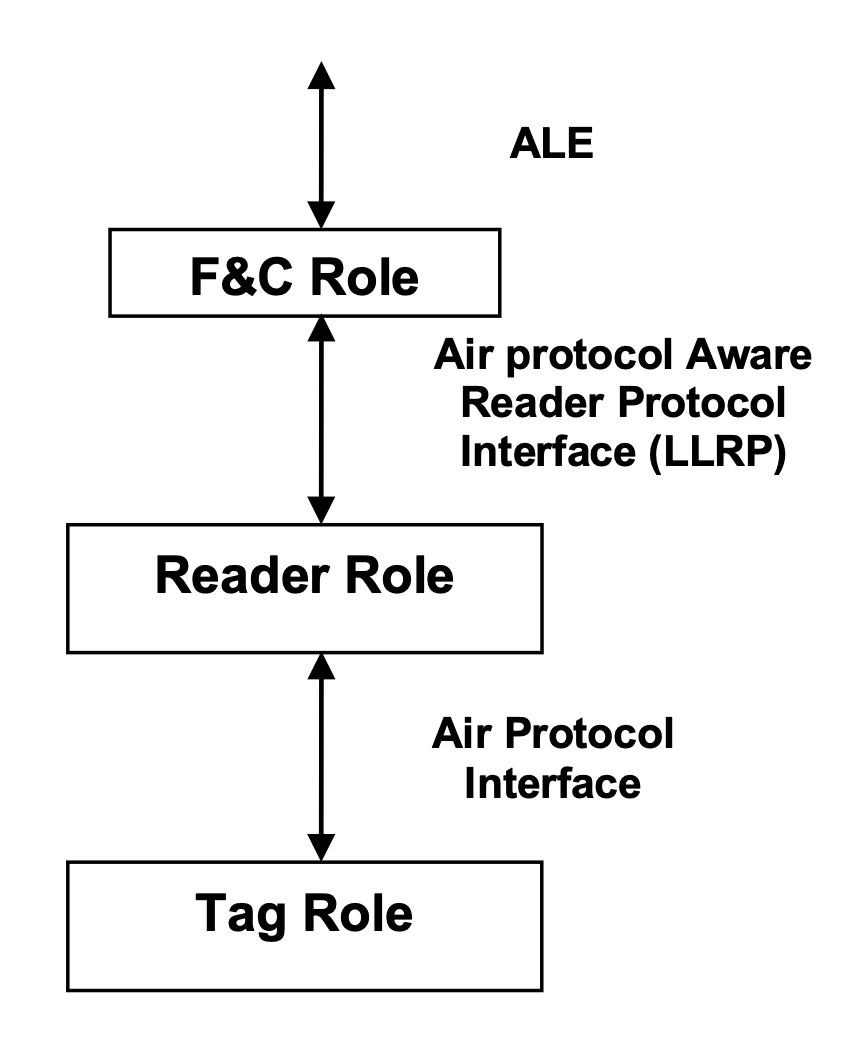
\includegraphics[width=0.4\textwidth]{./assets/02-state-of-the-art/llrp-interaction}
    \caption{\gls{LLRP} in the \emph{EPCglobal} Architecture~\cite{Llrp1standard20101013Pdf}} 
    \label{fig:02:llrp-interaction}
\end{figure}

\todo[inline]{Talk about LLRP for deployment of multiple readers e reader control and coordination?}

\section{Application Level Events (ALE)}

\section{EPCIS}

\todo[inline]{ver sec 5.1.1 da EPCISGuidelinePdf}

\section{EPCIS Capture Application}

\section{EPCIS Capture and Query Interfaces}

\section{EPCIS Repository}

\section{Core Business Vocabulary}

\section{Practical Context}

\todo[inline]{Nespresso supply-chain example and vision in the context of the EPCglobal framework, how it would work and advantages}
\chapter{Requirements and Development Options}

\section{System requirements}

\section{Manufacturers and development solutions}
\todo[inline]{Comparative analysis}

\section{Out choice}
\todo[inline]{Justification with a bit of detail}

\chapter{System Architecture and Development}

\section{Overall architecture}

\section{Hello World}
\todo[inline]{UHF Evaluation: Programs developed to evaluate the system, serialize and deserialize EPCs, Writing valid EPCs}

\section{Cloud and Modern Service Development}
\todo[inline]{Explain Linux containers, Docker and modern service development and deployment}

\section{RFID Serialization Plan}

\section{Identification Keys}

\section{Reader}

Octane 6.2.0 is based on LLRP version 1.0.1, which does not support C1G2 version 1.2.0.~\cite[sec. 3.1.21]{ImpinjOctaneLLRP}. Octane includes vendor extensions to expose the underlying air protocol features. For more information, refer to the documentation for the individual extensions.

\paragraph{ROBoundarySpec}

This parameter carries the lifetime of the Reader inventory and survey operation.
ROSpecStartTrigger, ROSpecStopTrigger: This is the start and stop trigger for this ROSpec.

Used ROSpecStopTriggerType Periodic.
Periodic trigger values: period - Time period specified in milliseconds; offset - Time offset specified in milliseconds from receiving message to start. useful for one-shot inventory.

Used ROSpecStartTriggerType Periodic.

\paragraph{Antenna inventory operations configuration (AISpec)}

AISpecStopTrigger parameter defines the stop (i.e., terminating boundary) of an antenna inventory operation~\cite[sec. 11.2.2.1]{Llrp1standard20101013Pdf}. Here it was set to Null to Stop when ROSpec is done.

InventoryParameterSpec Configuration (C1G2InventoryCommand) \dots

RF transmitter: Power, hoptableid, channelindex \dots

TagInventoryStateAware flag is used to determine how to process all the C1G2Filter and C1G2Singulation parameters in this command. At a functional level, if the Client is managing the tag states during an inventory operation (i.e., the Client is specifying Class1 Gen2 tag Select command Target and Action values), then it will set that flag to true and pass the appropriate fields in the C1G2 Filter and C1G2 Singulation parameters. If a reader set CanDoTagInventoryStateAwareSingulation to False in LLRPCapabilities (section 10.2.2), then the Reader SHALL ignore the TagInventoryStateAware flag.

The C1G2RFControl parameter~\cite[sec. 3.1.4]{ImpinjOctaneLLRP} specifies Speedway Gen2 modes selected by Impinj system engineering to provide the best performance. No Tari adjustment is necessary. Tari values passed by the client will be ignored.

Mode Index for the use case in this dissertation can be one of the three bellow, depending on the RF environment in which is deployed: 

- (the choice) 1002 (Autoset Static) configures the Reader to choose the best Gen2 link parameters for the environments where the tags population is relatively static and we wish to attempt to search for the weakest tag.

- 1003 (Autoset Static Fast) is an adaptation of Autoset Static for good RF environments

- 1004 (Autoset Static DRM) is an adaptation of Autoset Static for difficult RF environments

This C1G2SingulationControl Parameter provides controls particular to the singulation process in the C1G2 air protocol.

- Tag transit time**: This is the measure of expected tag mobility in the field of view of the antenna where this inventory operation is getting executed.
- **Tag population**: This is the expected tag population in the field of view of the antenna.
- **Session ID**: This is the C1G2 session number that the tags use to update the inventory state upon successful singulation.
- TagInventoryStateAwareSingulationAction: This is not used since the TagInventoryStateAware flag is set to false in the InventoryParameterSpec.

This parameters were not set to let the Impinj mode index use the optimal parameters.

\paragraph{Report Operation configuration (ROSpec)}

Describes the messages and parameters used in reports, event notifications and keepalives that are generated by the Reader and sent to the Client.

A reporting trigger (ROReportTrigger or AccessReportTrigger) generates a report while a connection is open.

In the use case in this dissertation we are not concerned with near real-time updates on the state of the inventory. So we can reduce the report generation by letting the end of the ROSpec generate a report periodically.
So ROReportTrigger can be set to Upon_N_Tags_Or_End_Of_ROSpec with N=0 (unlimited tag in antenna's field of view)~\cite[sec. 14.2.1]{Llrp1standard20101013Pdf}

In terms of the content useful to retrieve from the reader inventory singulation, the ROSpecID, FirstSeenTimestamp, LastSeenTimestamp are in the interests of the application.

We can enable it the TagReportContentSelector block by setting the Enable in each on.

\paragraph{Impinj Custom Parameters}

Impinj readers support Impinj extensions to the LLRP protocol. This extensions can be disabled by setting their values to zero. This will use the information defined in the LLRP parameters defined above.

One that is worth looking at is the ImpinjInventorySearchMode.
Impinj Readers implement state unaware singulation and therefore the Client does not control how the Reader attempts to singulate tags. This parameter provides a high-level control over the search algorithm and consequently does not interfere with any of the standard LLRP settings.~\cite[sec. 4.3.3]{ImpinjOctaneLLRP}
\todo[color=red]{rewrite}

Value 3, Single Target Inventory with Suppression (aka TagFocus), used for High tag count, high-throughput use cases where a reduction in repeated tag observations is acceptable. Suppresses repeated observations for extended periods of time while tags are energized. Supported only with Monza tags using Session 1. Since the we are using Monza R6-P tags, we can enable this mode.

\paragraph{Tools}

Used Fosstrak LLRP Commander with the old old Eclipse 3.3 and JRE/JDK1.8 to configure de reader using an xml schema.
Also developed a java tool to configure the reader using LLRP. Used the java llrp.ltk and code by impinj to configure it based on the "same" schema used in the LLRP commander.
In the java tool, the xml parser sometimes requires fields that shouldn't be needed because Impinj reader ignores then in certain configuration options. But for the configuration to be validated, they have to be present in order to validate de xsd schema (TagInventoryStateAware, Tari)

\section{Middleware}

\section{Capture application}

\section{EPCIS repository}

\section{Managements application}
\chapter{Test and evaluation}

\section{Laboratory tests}
\todo[inline]{Put and take}

\section{Range of operation tests}

\section{Operational tests}
\todo[inline]{Real case}
\chapter{Conclusion and Future Work}

\section{Retell the story from motivation to results}

\section{Main achievements}

\section{Future Work}

% Back cover, bibliography and attachments
\bibliographystyle{unsrt}
\bibliography{biblio.bib}
%\cleardoublepage

\end{document}
